% BEGIN_FOLD
\documentclass[a4paper,11pt]{report} % Sets the documentclass
\usepackage[english]{babel} 	% Ordbog
\usepackage[utf8]{inputenc}	% No idea
\usepackage{graphicx} 	   	% Makes graphics to the document
\usepackage{mathtools} 		% Enables mathmode
\usepackage{float}	 	% Lets you place graphics for example
\usepackage{fancyhdr} 		% Package for footers and headers
\usepackage[font=small, font=it, labelfont=bf]{caption} 		% Gives extra manipulation of captions
\usepackage[font=small, font=it, labelfont=bf]{subcaption} 	% Lets you put captions in for example subfigures
\usepackage{wrapfig} 		% Lets you "wrap" text around figures and tables
\usepackage{comment} 		% Text between \comment and \endcomment is discarded
\usepackage{amsmath} 		% Math environment
\numberwithin{equation}{section}
\usepackage{color} 		% Lets you add color to text
\usepackage{hyperref} 		% Reference pages, sections, figure etc. and directly link to them
\usepackage{titlesec} 		% Adds a lot of diffrent new manipulations with titles, headers and contents.
\usepackage{grffile}
\usepackage[table]{xcolor} 	% Giver mulighed for at give tabeller farve
\usepackage[sorting=none]{biblatex}
\usepackage{listings}
\usepackage{tikz} % Flowcharts and vector drawings
\usepackage{url}
\usepackage{breqn}
\usepackage{array}
\usepackage{placeins} % Allows for FloatBarrier
\usepackage{csquotes}

%% Looks of document
%\usepackage[margin=1.3in]{geometry}

%% bibliography

\addbibresource{bib/masterBib.bib}
%\bibliography{MasterBibs}


%% General Document graphics:
\setcounter{secnumdepth}{4} 	% Sets numbering to maximum the fourth subsection
\setcounter{tocdepth}{2} 	% Laver indholdsfortegnelse med en dybde på 2 underafsnit
\pagestyle{plain} 		% Lader dig placere sidenummer. Others are for example empty or myheadings. 
%\usepackage{fullpage} 		% Gør marginerne mindre i forhold til standard.
%\usepackage[margin=0.8in]{geometry} % Ændre på margins størrelse.


\definecolor{darkred}{RGB}{180,20,20}

% END_FOLD

\usepackage{printlen}

\begin{document}

\uselengthunit{cm}\printlength{\textwidth}

\title{Cross Immunity in Stochastic, Agent-based Malaria Model}
\author{Jeppe Finne Sørensen \\ gtc329@alumni.ku.dk \\ 06-02-1993}
\date{Masters Project \\ KU; Niels Bohr Institute \\ 10. of September}

\maketitle
\thispagestyle{empty}

\newpage	

\chapter{Python Figures}

In the next section, python figures will be shown.

\section{The python figures}

\begin{figure}
	\centering
	\begin{subfigure}{0.49\textwidth}
		\centering
		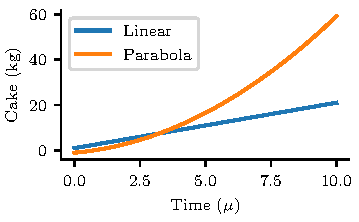
\includegraphics[width=1\linewidth]{fig/TwoGolden.pdf}
		\caption{}
	\end{subfigure}
	\begin{subfigure}{0.49\textwidth}
		\centering
		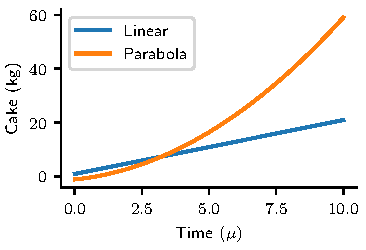
\includegraphics[width=1\linewidth]{fig/TwoInnerGolden.pdf}
		\caption{}
	\end{subfigure}
	\caption{}
\end{figure}

\begin{figure}
\centering
\begin{subfigure}{0.8\textwidth}
	\centering
	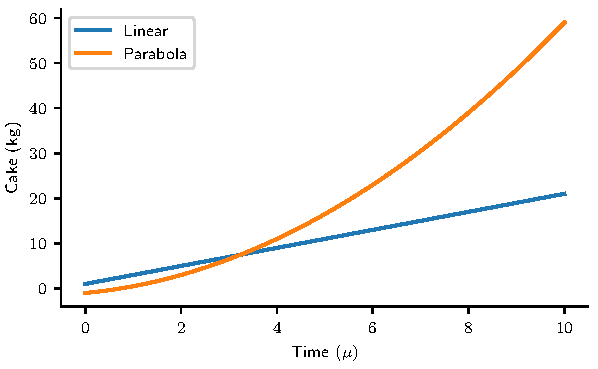
\includegraphics[width=1\linewidth]{fig/OneGoldenSmall.pdf}
	\caption{}
\end{subfigure}
\caption{}
\end{figure}

\begin{figure}
\centering
\begin{subfigure}{0.99\textwidth}
	\centering
	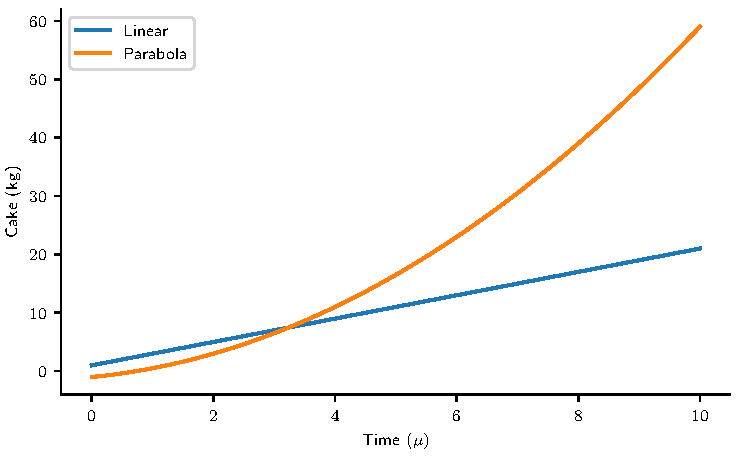
\includegraphics[width=1\linewidth]{fig/OneGoldenFull.pdf}
	\caption{}
\end{subfigure}
\caption{}
\end{figure}

\end{document}